\subsubsection{01.03.2016}
\textit{\textbf{Time frame:}} 17:30-21:30 

It was held the investigation on the most convenient way of constructing the lifting mechanism. The aim was to find the construction, which would be able to withstand twisting force caused by the shifted to the side bucket with debris.

There was tested a number of constructions and it was investigated that construction with two rails at the angle of $90^\circ$ provides the best resistance to the twist. Unfortunately, only to the one side (figure \ref{Elevator4.3}, \ref{Elevator4.4}).

\begin{figure}[H]
	\begin{minipage}[h]{0.47\linewidth}
		\center{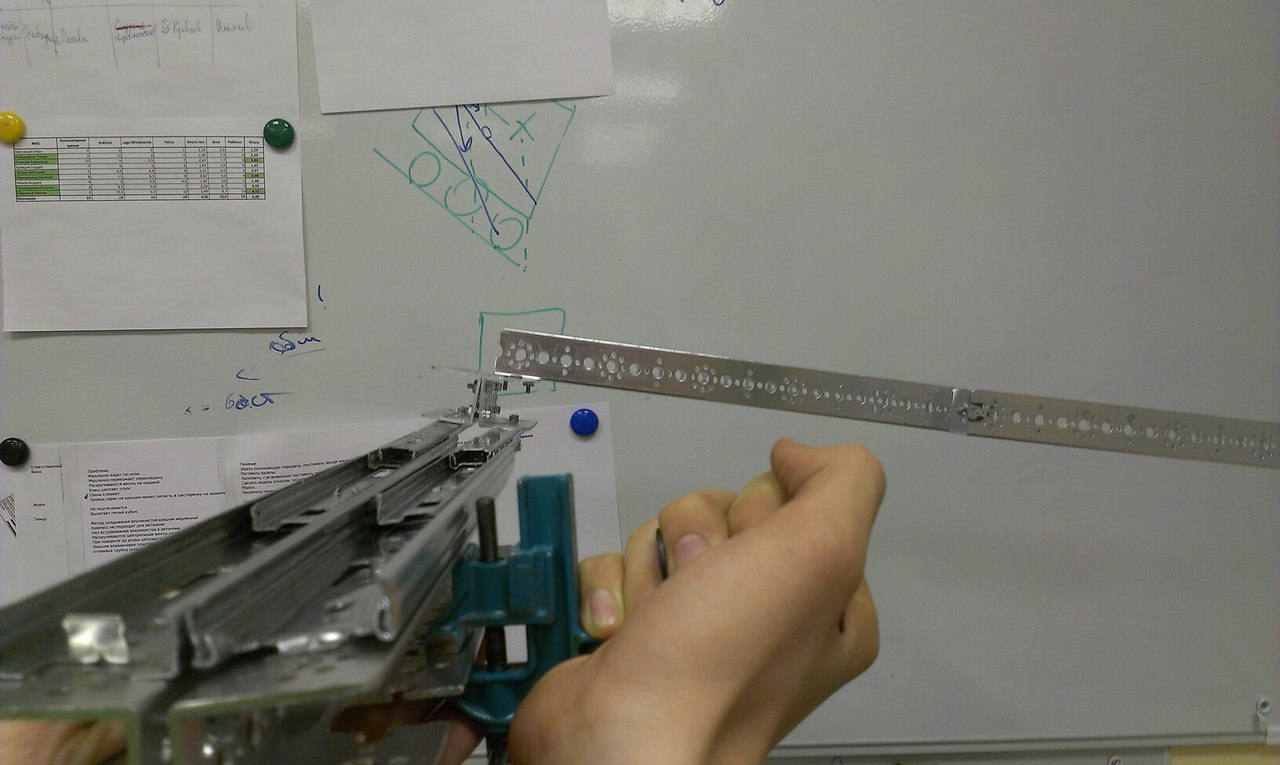
\includegraphics[scale=0.2]{3Engineering/5Team_meetings/days_of_meetings/2016.03.01/images/01}}
		\caption{Two parallel rails}
		\label{Elevator4.1}
	\end{minipage}
	\hfill
	\begin{minipage}[h]{0.47\linewidth}
		\center{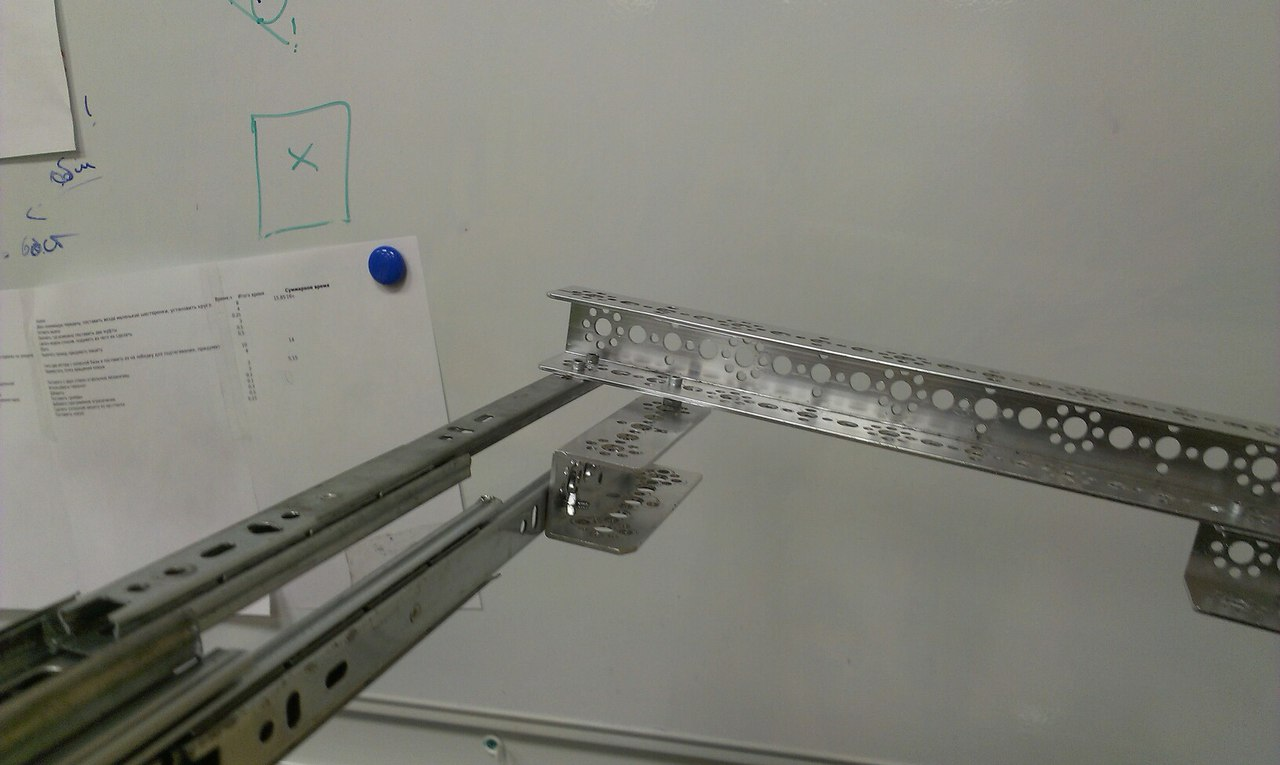
\includegraphics[scale=0.2]{3Engineering/5Team_meetings/days_of_meetings/2016.03.01/images/03}}
		\caption{One rail turned on $90^\circ$}
		\label{Elevator4.2}
	\end{minipage}
	\vfill
	\begin{minipage}[h]{0.47\linewidth}
		\center{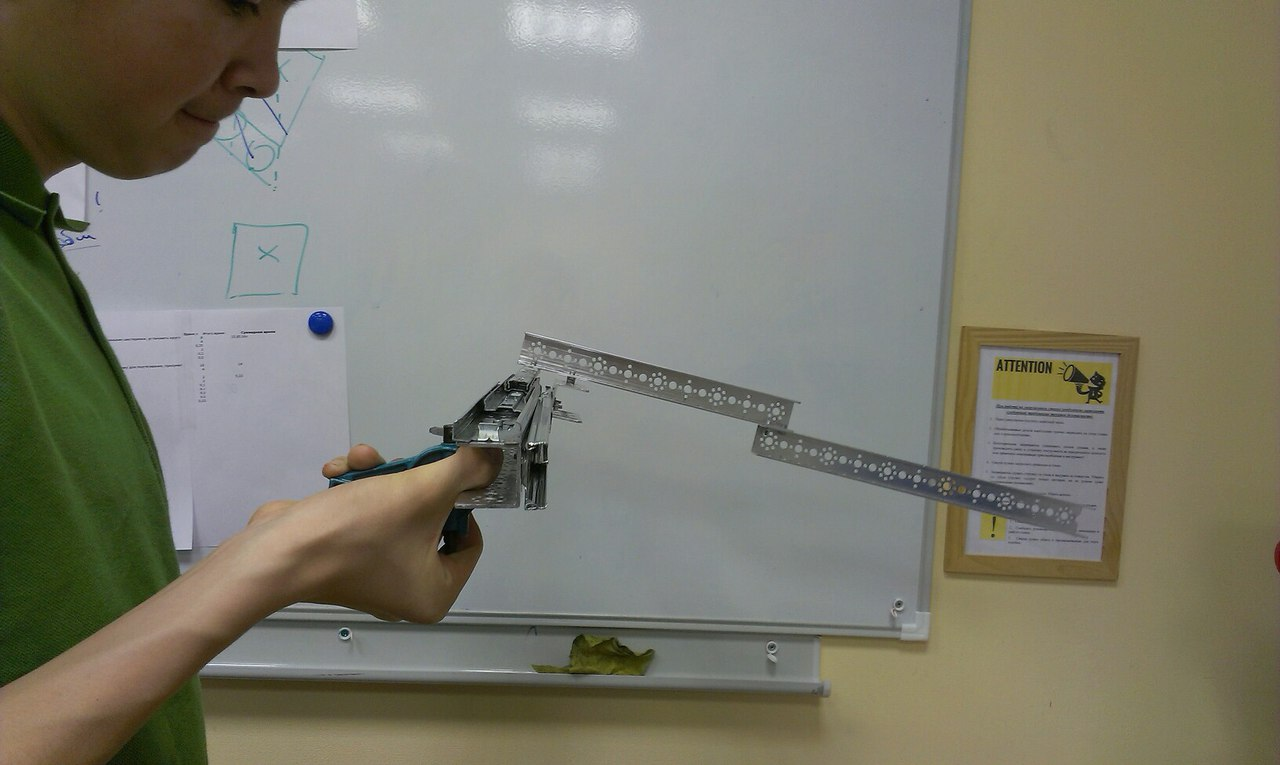
\includegraphics[scale=0.2]{3Engineering/5Team_meetings/days_of_meetings/2016.03.01/images/02}}
		\caption{One rail turned on $90^\circ$ (testing right bend)}
		\label{Elevator4.3}
	\end{minipage}
	\hfill
	\begin{minipage}[h]{0.47\linewidth}
		\center{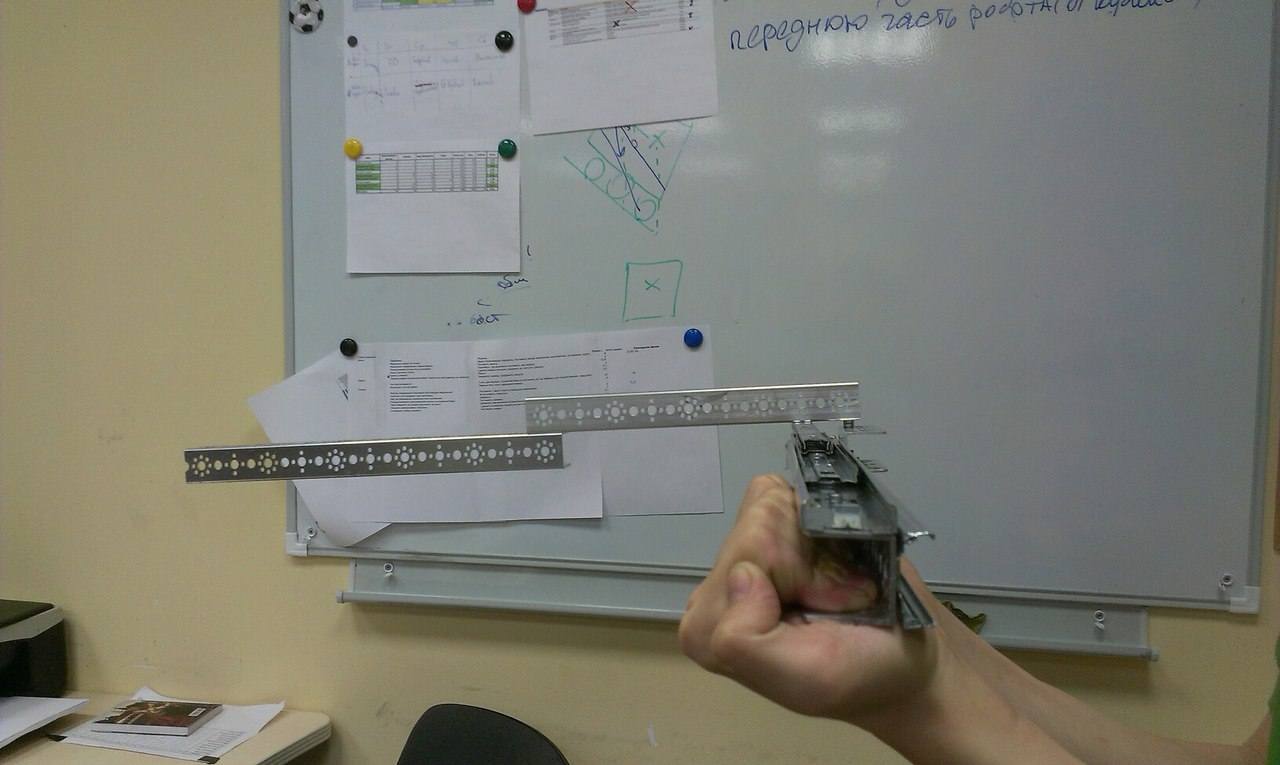
\includegraphics[scale=0.2]{3Engineering/5Team_meetings/days_of_meetings/2016.03.01/images/04}}
		\caption{One rail turned on $90^\circ$ (testing left bend)}
		\label{Elevator4.4}
	\end{minipage}
\end{figure}

